\documentclass{article}
\usepackage{graphicx} % Required for inserting images
\usepackage{float}
\usepackage[english]{babel}
\usepackage{amsthm}
\usepackage{amsmath}
\DeclareMathOperator*{\argmin}{arg\,min}
\usepackage{amsfonts}
\usepackage{amssymb}
\usepackage{tabularx}
% MLA change this
\usepackage[sorting=none]{biblatex}
\usepackage{csquotes}
\usepackage[dvipsnames]{xcolor}


\addbibresource{custom.bib}

\theoremstyle{definition}
\newtheorem{definition}{Definition}[section]
\newtheorem{theorem}{Theorem}[section]

\title{Extended Essay - Mathematics \\[1ex] 
\author{} 
\large To what extent does the activation function of a neural network impact the smoothness and curvature of its loss function?}
\date{}
\begin{document}
%TC:ignore
\maketitle
\clearpage
\tableofcontents
\clearpage
\section{Introduction}
%TC:endignore
Neural networks have captivated the world with their ability to accurately automate data-driven tasks like classification and generation. Recent advancements in generative Artificial Intelligence (AI), including large language models like ChatGPT, have ensured the modern-day ubiquity of these deep and complex networks \cite{nature_deep_learning}. This motivates the need to better understand the underlying mechanisms behind AI technology to optimize a tool used by millions  \cite{ai_usage_stats}. This essay focuses on foundational neural networks used for binary classification. These represent smaller-scale models whose parameters allow for exploration and whose size permits easy experimentation.


Since most neural networks have similar architectures, mathematical models employed in this essay, like multivariable calculus, real analysis, and linear algebra, apply to larger networks. These tools provide insights into function curvature and higher-dimensional spaces. They also strongly correlate with training stability and performance when applied to network areas like activation and loss functions. Therefore, this essay addresses the following research question: \textit{To what extent does the activation function of a neural network impact the smoothness and curvature of its loss function?}

%TC:ignore
\section{Properties of Neural Networks}
\subsection{Structure}
%TC:endignore

As the name suggests, neural networks are loosely modeled on the human brain \cite{ai_bio}. Both systems contain information-storing nodes, known as neurons, that learn data patterns through transfers and transformations of information with other neurons in distinct layers. Through exposure to larger information sets, allowing for careful calibration of neural connections, both systems gradually improve performance on data-based tasks.

Most advanced AI technologies use deep neural networks. These models pass input features through multiple neuronal layers, known as hidden layers, rather than directly transforming inputs into outputs. Deep networks allow for more neural connections with the potential to learn complex relationships. 

\begin{figure}[H]
    \centering
    \includegraphics[width=1\linewidth]{basic_nn.png}
    \caption{Simplified structure of deep neural networks \cite{nn_book}}
    \label{fig:Figure 1}
\end{figure}

Although hidden layers, seen in Figure~\ref{fig:Figure 1}, can contain an arbitrary number of neurons, output layers  contain just one neuron in binary classifiers. If an output neuron's prediction is larger than a set threshold, typically between zero and one, the model will  positively classify input features. 
\begin{definition}[Binary Classifier]
\label{bclassdefinition}
Let $\hat{y}$ represent the prediction held by the output neuron in a binary classifier. The possible outcomes for binary classification, depending on a set numerical threshold, are given by:

\begin{equation*}
outputs = \begin{cases}
0,  \hat{y} \leq threshold \\
1,  \hat{y} > threshold
\end{cases}
\end{equation*}

\end{definition}
Between layers, a neuron's value ($a$) is transformed using a weight, bias, and an activation function. Weights ($w$) and biases ($b$) apply a linear weighted sum on neuronal values in the form $wa + b$. Furthermore, an activation function adds key nonlinearities to the network, the importance of which is analyzed in Section~\ref{sec:activation}. The equation for a  connection between a neuron and its preceding layer with $k$ total neurons is therefore given by:

\begin{equation}
\label{eq:first_nn_eq}
\begin{aligned}
a_i^{(j)} &= \sigma(\Vec{w}^{(j)}_i \cdot \Vec{a}^{(j-1)} + b^{(j)}_i) \\
\Vec{w}^{(j)}_i &\in \mathbb{R}^{k},\quad b^{(j)}_i \in \mathbb{R}^1,\Vec{a}^{(j-1)} \in \mathbb{R}^{k}, a_i^{(j)} \in \mathbb{R}^1
\end{aligned}
\end{equation}
Where $a_i^{(j)}$ represents a neuron value (known as an activation) in the j\text{th} layer, $w_i$ represents the weight vector of all incoming features to $a_i^{(j)}$, $b_i$ represents an added bias term, and $\sigma(x)$ is the non-linear activation function. The index $i$  indicates that the connection between one specific neuron (the ith neuron in the layer) is being analyzed. 
Since this weighted sum is applied at every network connection, Equation~\eqref{eq:first_nn_eq} must be generalized to include the transformations of the entire network at a particular layer. Notationally, this can be achieved by representing a neural network as a large matrix-vector multiplication \cite{3blue1brown_nn}. 
\begin{definition}[Weighted Sums of Layered Connections]

Let \( W \) represent the matrix of weights connecting a layer with \( k \) neurons to a layer with \( n \) neurons:
\[
W^{(j)} =
\begin{bmatrix}
w_{0,0} & w_{0,1} & \cdots & w_{0,n} \\
w_{1,0} & w_{1,1} & \cdots & w_{1,n} \\
\vdots & \vdots & \ddots & \vdots \\
w_{k,0} & w_{k,1} & \cdots & w_{k,n}
\end{bmatrix}
\]

%$W^{(j)} \in \mathbb{R}^{k,n}$

Furthermore, let \( A^{(j)} \) represent a vector holding all neuron data in the \( j\)-th layer:

\[
A^{(j)} = 
\begin{bmatrix}
a^{(j)}_0 \\
a^{(j)}_1 \\
\vdots \\
a^{(j)}_k
\end{bmatrix}
\]

Finally, let \( b \) represent a vector with all the bias terms in the same layer:
\[
b = 
\begin{bmatrix}
b_0 \\
b_1 \\
\vdots \\
b_n
\end{bmatrix}
\]

We have that:
\begin{equation}
\label{eq:nn_eq}
A^{(j)} = \sigma(W^T A^{(j-1)} + b)
\end{equation}

\end{definition}
Definition 2.2 yields an entire weight matrix and bias vector to transform data. These weights and biases are tunable parameters in every neural network. Model training involves discovering a set of weights and biases that map input features to output expectations most accurately. 

In fact, neural networks are universal approximators \cite{uat}. A universal approximator is defined as a method that approximates any function to within an arbitrarily tiny margin of error $\epsilon$. This intrinsic property of neural networks underscores their usefulness, owing to their theoretical ability to represent any mathematical relationship. 

% \begin{theorem}[Universal Approximation Theorem]
% Let $I^n$ represent the input space to a neural network that contains a vector of continuous real numbers. The valid set of function spaces for a neural network is therefore given by:
% \[
% C(I^n) = \{f:I^n \xrightarrow[]{} \mathbb{R} \: |\text{ $f$ is continuous}\}
% \]
% Let the supremum norm of function $f$ be defined by the following operation:
% \[
% ||f||_\infty = \sup_{x \, \in \, I^n}|f(x)|
% \]
% Finally, let us define a neural network function, $F$, which computes the weighted sums of the entire neural network. $F$ is characterized by one hidden layer with $m$ hidden neurons and an arbitrary non-linear activation function $\sigma : \mathbb{R} \xrightarrow[]{} \mathbb{R}$:
% \[
% \begin{aligned}
% F_{m, \sigma}(x) = \sum_{j=1}^{m} \: \alpha_j \: \sigma(w_j^Tx+b_j) + c \\
% x \in I^n, \{a_j, c, b_j\} \in \mathbb{R}, w_j \in \mathbb{R}^n
% \end{aligned}
% \]
% This definition of $F$ condenses weighted sum computations for two layers, as defined earlier by Equation~\ref{eq:nn_eq}, into one calculation to map out the entire three-layered network, summing across all the neurons in our arbitrarily sized hidden layer. We now formalize this definition by stating that this neural network architecture is one of numerous possible functions that can transform input to output in the conditions defined in our $C(I^n)$ space:
% \[
% H_{\sigma} = \{F_{m, \sigma} \: | m \in \mathbb{N}, a_j, c, b_j, w_j\} \subseteq C(I^n)
% \]
% Now, assume that $\sigma$ is bounded, continuous, and non-polynomial. For every $f \in C(I^n)$ and every $\epsilon > 0$, there exists a network $F \in H_{\sigma}$ such that:
% \[
% ||f-F||_\infty < \epsilon
% \]
% Thus, no matter how we choose an error rate $\epsilon$, a neural network can always approximate a function with higher accuracy than that rate. Coming close to finding this ideal network requires a quantitative understanding of network performance through metrics such as loss.
% \end{theorem}

%TC:ignore
\subsection{Loss Function}
\label{sec:lossfunc}
%TC:endignore
To evaluate the accuracy of a neural network, a loss function is used. This function quantifies differences between network outputs and expected outputs, averaged across all test cases.
The loss function used in this essay is Negative Log Likelihood, given by:
\begin{equation}
L(y, p^*) = - \frac{1}{N} \sum_{i=1}^N (y_i\ln(p^*_i) + (1-y_i)\ln(1-p^*_i))
\end{equation}
Where $y_i$ represents the desired output for a given test instance $i$, $p_i^*$ represents the model's predicted output for the same instance, and $N$ represents the total number of such instances the model is being measured against.
For a binary classifier, Negative Log Likelihood is the loss function whose optimum represents a maximum likelihood estimator for any input data \cite{mll}. This is under the (typically true) assumptions that every test case occurs independently, and that all test cases have been derived from the same data generation process. 
\begin{definition}(Maximum Likelihood Estimator)
Let $H$ represent the hypothesis space of a neural network, with $\theta$ representing a specific set of parameters in this hypothesis space. Maximum likelihood estimation involves finding a $\theta^*$ that best fits the distribution of a given $H$. Minimizing the Negative Log Likelihood function directly corresponds to increasing neural network probabilities for correct data classifications. 
\end{definition}
\begin{proof}
Let $y_i \in \{0,1\}$ represent the desired output for a specific instance of a neural network, with inputs represented by $x_i$ and free parameters (weights and biases) represented by $\theta$. A maximum likelihood estimator draws from a Bernoulli distribution to model the network's binary classification capabilities.\\ \\ Using $P(y_i = 1\:|\: x_i\,;\,\theta)$, the likelihood that a binary classifier predicts positively given its inputs, we have:
\[
P(y_i = 1\:|\: x_i\,;\,\theta) = P(y_i = 1\:|\:x_i \, ; \, \theta)^{y_i} \cdot (1-P(y_i = 1\:|\:x_i \, ; \, \theta))^{1-y_i}
\]
Let $p^*_i = P(y_i = 1 \, | \, x_i \, ; \, \theta)$ represent the probability that the model outputs the positive binary class, and let $L(y, p^*)$ represent the loss function. Since we assume each test case is independent, the following can be performed across $N$ test cases:
\[
L(y, p^*) = \prod^N_{i=1}(p^*_i)^{y_i} \cdot (1-p^*_i)^{1-y_i}
\]
To simplify the above expression, we can take logarithms of both sides. This will transform the product expression into a summation without altering the relative values of probabilities, since the logarithmic function monotonically increases between 0 and 1 (domain of all probabilities):
\begin{equation*}
\begin{aligned}
ln(L(y, p^*)) &= \sum_{i=1}^N \: \ln[(p^*_i)^{y_i} \cdot (1-p^*_i)^{1-y_i}] \\
&= \sum_{i=1}^N \: \ln[(p^*_i)^{y_i}] + \ln[(1-p^*_i)^{1-y_i}]\\
&= \sum_{i=1}^N \: y_i[\ln(p^*_i)] + (1-y_i)\ln[(1-p^*_i)]
\end{aligned}
\end{equation*}

This represents the likelihood the network is aiming to maximize. For the converse, the loss statement, we have:
\begin{equation*}
\begin{aligned}
&-\ln(L(y, p^*)) = - \sum_{i=1}^N (y_i\ln(p^*_i) + (1-y_i)\ln(1-p^*_i)) \\
&\theta^* = \argmin_{\theta^*}(-\ln(L(y, p^*)))
\end{aligned}
\end{equation*}
An exact match with the loss function in Equation~\eqref{eq:nn_eq}. 
\end{proof}
\subsection{Gradient Descent and Backpropagation}
\label{sec:grad_desc}
Given the above architecture, training a network involves finding a local loss minimum by optimizing weight and bias parameters. The multidimensionality of loss surfaces (involving hundreds or thousands of tunable parameters), combined with their non-convex nature, makes finding a global minimum difficult and computationally inefficient. Local minima with high classification accuracies are sufficient.

Gradient descent is the most popular technique for finding these minima. It uses a gradient vector to differentiate the loss function with respect to every network parameter. With this vector, the technique continually moves a network's position on its loss surface until a local minimum is reached. Formally, gradient descent is given by:
\begin{equation}
\label{eq:gradient_descent}
    \Delta v = - \eta \nabla C
\end{equation}
Where $\Delta v$ represents the change in position on the loss surface, $\nabla C$ is the gradient vector, and $\eta$ is the learning rate, a hyperparameter that scales step size. This technique requires multiple steps to successfully minimize loss, as seen in Figure~\ref{fig:Figure 2}, where simplified gradient descent is shown for one parameter.
%TC:ignore
\begin{figure}[H]
    \centering
    \includegraphics[width=1\linewidth]{gradient_descent.jpg}
    \caption{Depiction of single-variable gradient descent \cite{gradesc}}
    \label{fig:Figure 2}
\end{figure}
%TC:endignore
To repeatedly apply Equation~\eqref{eq:gradient_descent}, the network's gradient vector ($\nabla C$) must be updated at each step. This process relies on another key algorithm, backpropagation, which differentiates the loss function with respect to every network parameter.
\begin{definition}(Backpropagation)
To update the $\nabla C$, the backpropagation algorithm must calculate $\frac{\partial C_0}{\partial W^{(L)}}$, where $C_0$ represents the loss function for a given training example, and $W^{(L)}$ represents the weight matrix for connecting a given layer with its previous layer. This algorithm is repeatedly applied across network layers to calculate the full gradient vector. 
\end{definition}
\begin{proof}
Recall Equation~\eqref{eq:nn_eq}, which defines a neural network weighted sum by:
\[
A^{(L)} = \sigma(WA^{(L-1)} + b)
\]
Furthermore, assume $Z^{(L)} = (WA^{(L-1)} + b$).
By the chain rule, we have that:
\[
\frac{\partial C_0}{\partial W^{(L)}} = \frac{\partial Z^{(L)}}{\partial W^{(L)}} \cdot \frac{\partial A^{(L)}}{\partial Z^{(L)}} \cdot \frac{\partial C_0}{\partial A^{(L)}}
\]
Though the partial derivatives here differentiate entire vectors (such as $A^{(L)}$) and matrices (such as $W^{L}$), the above equation is used for notational simplicity. The result is a Jacobian matrix (a matrix of first derivatives of a vector-valued function) equivalent in size to the weight matrix. \\ \\
Recall from our definition of a non-activated weighted sum, $Z^{(L)}$, that its derivative is equal to the activations in the previous layer (due to linearity):
\[
\frac{\partial Z^{(L)}}{\partial W^{(L)}} = A^{(L-1)}
\]
Furthermore, recall that the equation of a neural network is given by $A^{(L)} = \sigma (Z^{(L)})$. Therefore:
\[
\frac{\partial A^{(L)}}{\partial Z^{(L)}} = \sigma'(Z^{L})
\]
Finally, given our loss function $L(y, p^*)$, we have $p^*$ representing a model prediction at any given layer, which is equal to $A^{(L)}$. As a result:
\[
\frac{\partial C_0}{\partial A^{(L)}} = C'(y, A^{(L)})
\]
With C representing the restated loss function. Combining these intermediates, we have:
\[
\frac{\partial C_0}{\partial W^{(L)}} = A^{(L-1)} \cdot \sigma'(Z^{L}) \cdot C'(y, A^{(L)})
\]
Averaging across $n$ training examples, we obtain our complete cost function derivative with respect to a specific weight:
\[
\frac{\partial C}{\partial W^{(L)}} = \frac{1}{n} \sum_{k = 0}^{n-1} \frac{\partial C_k}{\partial W^{(L)}}
\]
Arranging these partial derivatives into the gradient vector, we have:
\[
\nabla C =
\begin{bmatrix}
\frac{\partial C}{\partial W^{(1)}} \\
\vdots \\
\frac{\partial C}{\partial W^{(L)}}
\end{bmatrix}
\]
For $L$ layers in the neural network. \\ \\
Here, each vector entry is a Jacobian matrix, holding loss derivatives of network weights per layer. Since different layers contain different numbers of weights (leading to non-uniform matrix sizes), these Jacobians are listed as separate entries of $\nabla C$. 
\end{proof}

%TC:ignore
\section{Activation Functions}
\label{sec:activation}
\subsection{The Need for Nonlinearities}
%TC:endignore
As mentioned, activation functions significantly determine the training stability and speed of a neural network. They are essential to any architecture, as these functions add nonlinearities to weighted sums computed between each neuron connection. 
Consider a neural network without an activation function. Its weighted sum at a single connection is given by the linear equation:
\[
A^{(L)} = W^{(L)}A^{(L-1)} + b^{(L)}
\]

Now, consider the weighted sum for the same neuron in the next layer:
\[
A^{(L+1)} = W^{(L+1)}A^{(L)} + b^{(L+1)}
\]

By substitution, we have:
\[
A^{(L+1)} = W^{(L+1)} \cdot [W^{(L)}A^{(L-1)} + b^{(L)}] + b^{(L+1)}
\]

Let $M = W^{(L+1)}\cdot W^{(L)}$ and $C = W^{(L+1)} \cdot b^{(L)} + b^{(L+1)}$. We have that:
\[
A^{(L+1)} = MA^{(L-1)} + C
\]
Without an activation function, our entire network becomes a large composition of linear functions, resulting in strictly linear outputs. Nonlinearities obtained through an activation function are essential in ensuring that a network has the capacity to learn patterns that are more complex than linear relationships. 
%TC:ignore
\subsection{Sigmoid}
%TC:endignore
Among the earliest and most popularly used activation functions is sigmoid, or the logistic curve. This is a function bounded on the interval $(0, 1)$, given by the equation:
\begin{equation}
\label{sigmoid}
S(x) = \frac{1}{1+e^{-x}}
\end{equation}
%TC:ignore
\begin{figure}[H]
    \centering
    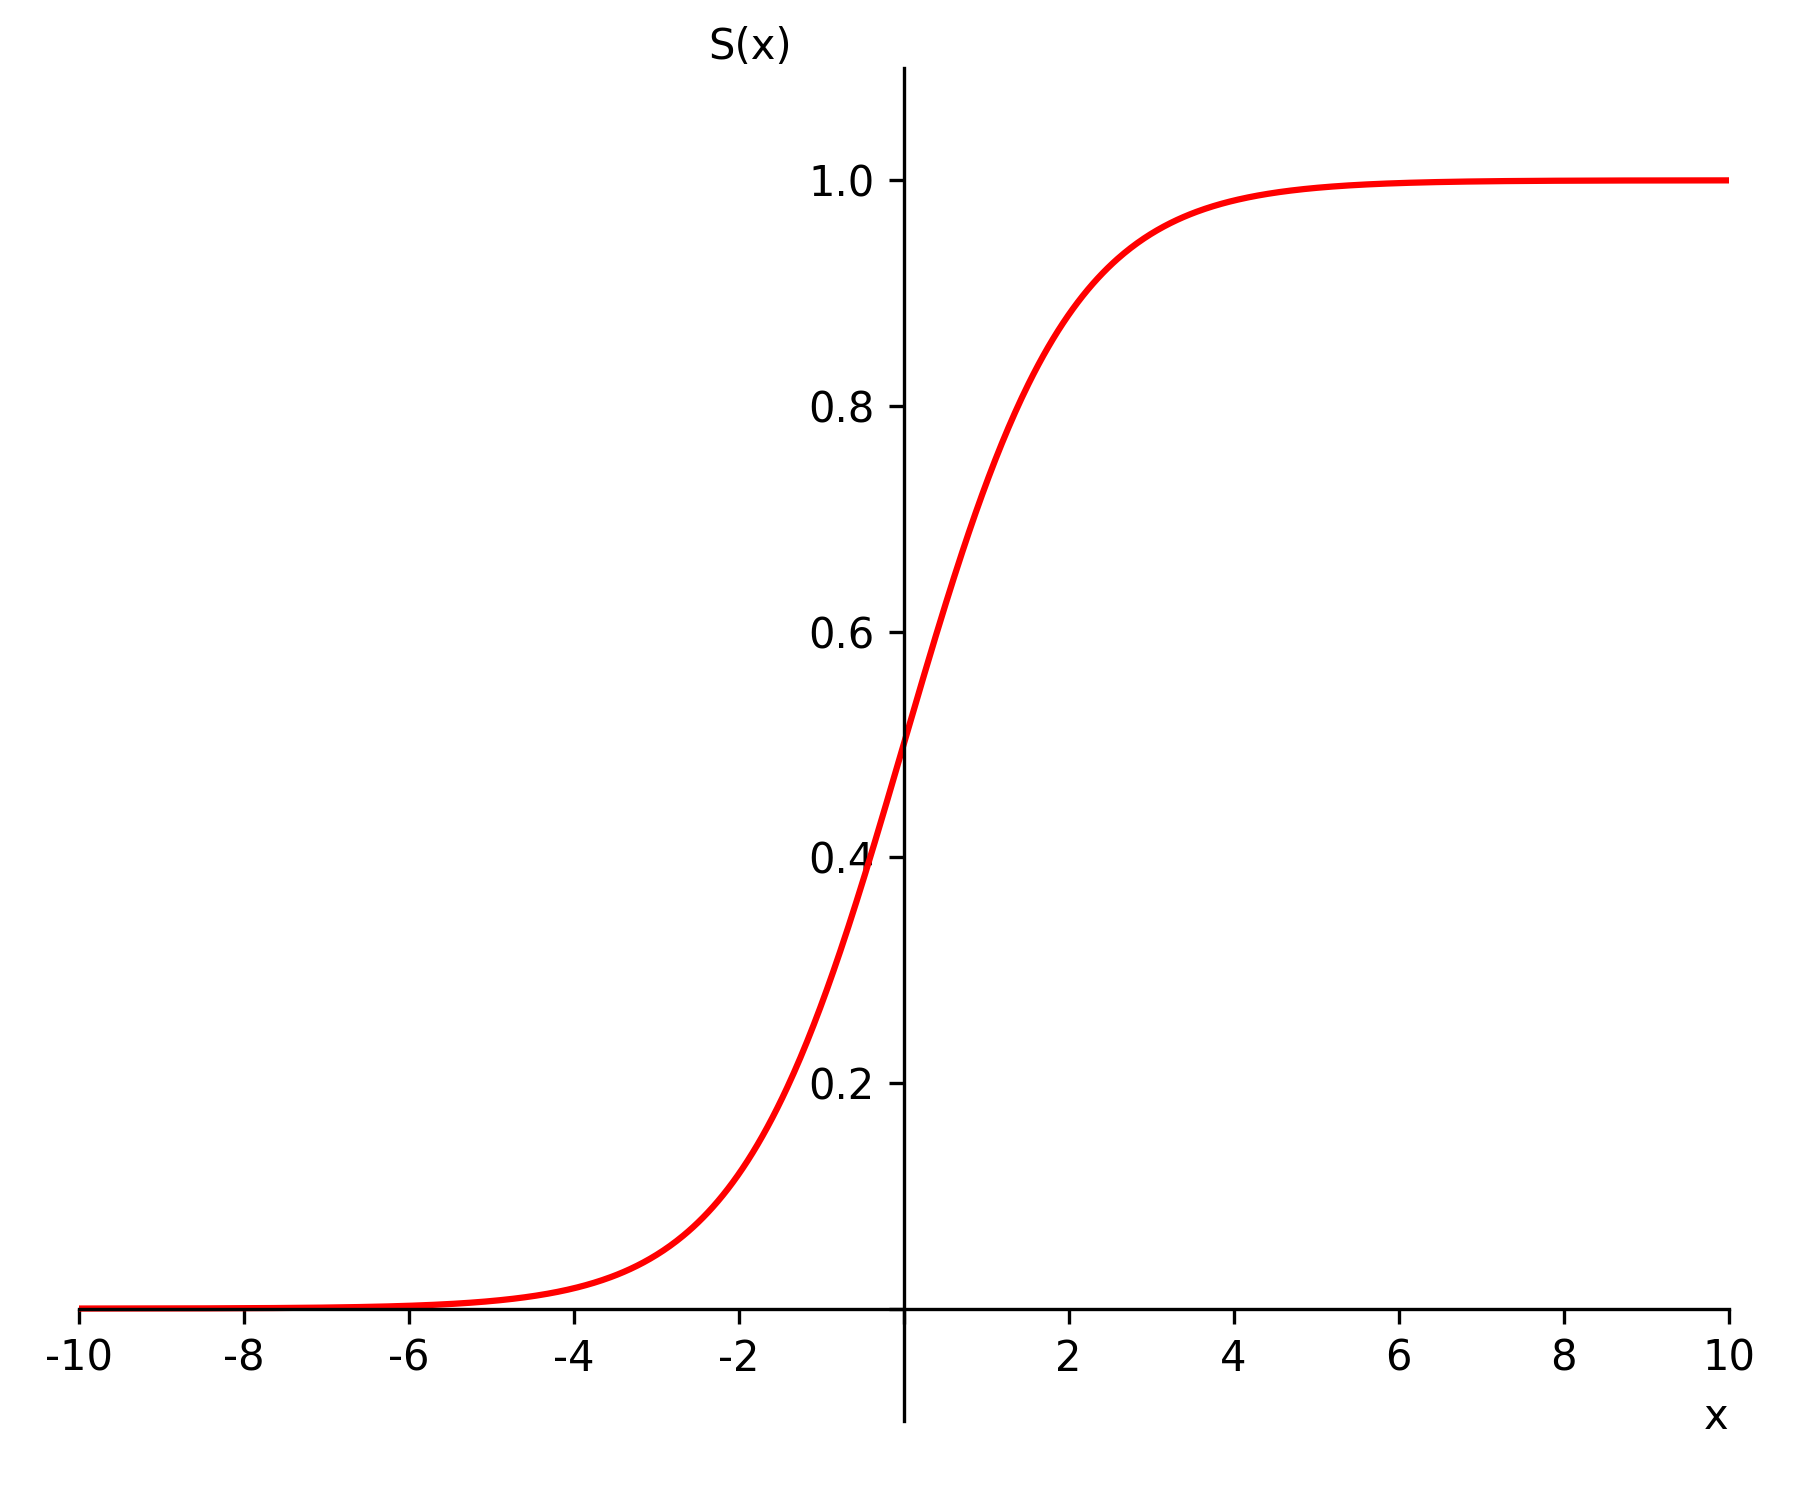
\includegraphics[width=1\linewidth]{Sigmoid.png}
    \caption{Sigmoid function}
    \label{fig:Figure 3}
\end{figure}
%TC:endignore
Curve bounds intrinsically render sigmoid a useful binary classifier. By always outputting a value between zero and one, the function mimics the classification threshold outlined in Definition~\ref{bclassdefinition}. Owing to these matching limits, output layers in binary classifiers always use the logistic curve as an activation function. The key is to identify whether sigmoid continues to benefit in preceding layers.

The rate of change of the logistic curve helps understand its role in activating neural connections.
\begin{definition}[Derivative of Sigmoid]
    By the quotient rule, we have that:
    \[
        S^{'}(x)=\frac{-\frac{d}{dx} (1+e^{-x})}{(1+e^{-x})^2}
    \]
    From the chain rule, we have:
    \[
        \frac{d}{dx} (1+e^{-x})= -e^{-x}
    \]
    Substituting back:
    \[
        S'(x)=\frac{e^{-x}}{(1+e^{-x})^2}
    \]
    Expressed in terms of the original function:
    \[
        1-S(x) = \frac{e^{-x}}{(1+e^{-x})}
    \]
    \[
        S'(x) = S(x)(1-S(x))
    \]
\end{definition}
Due to curve bounds, causing multiplication of decimals between zero and one, the derivative of sigmoid will always be lower than its base function output.
%TC:ignore
\begin{figure}[H]
    \centering
    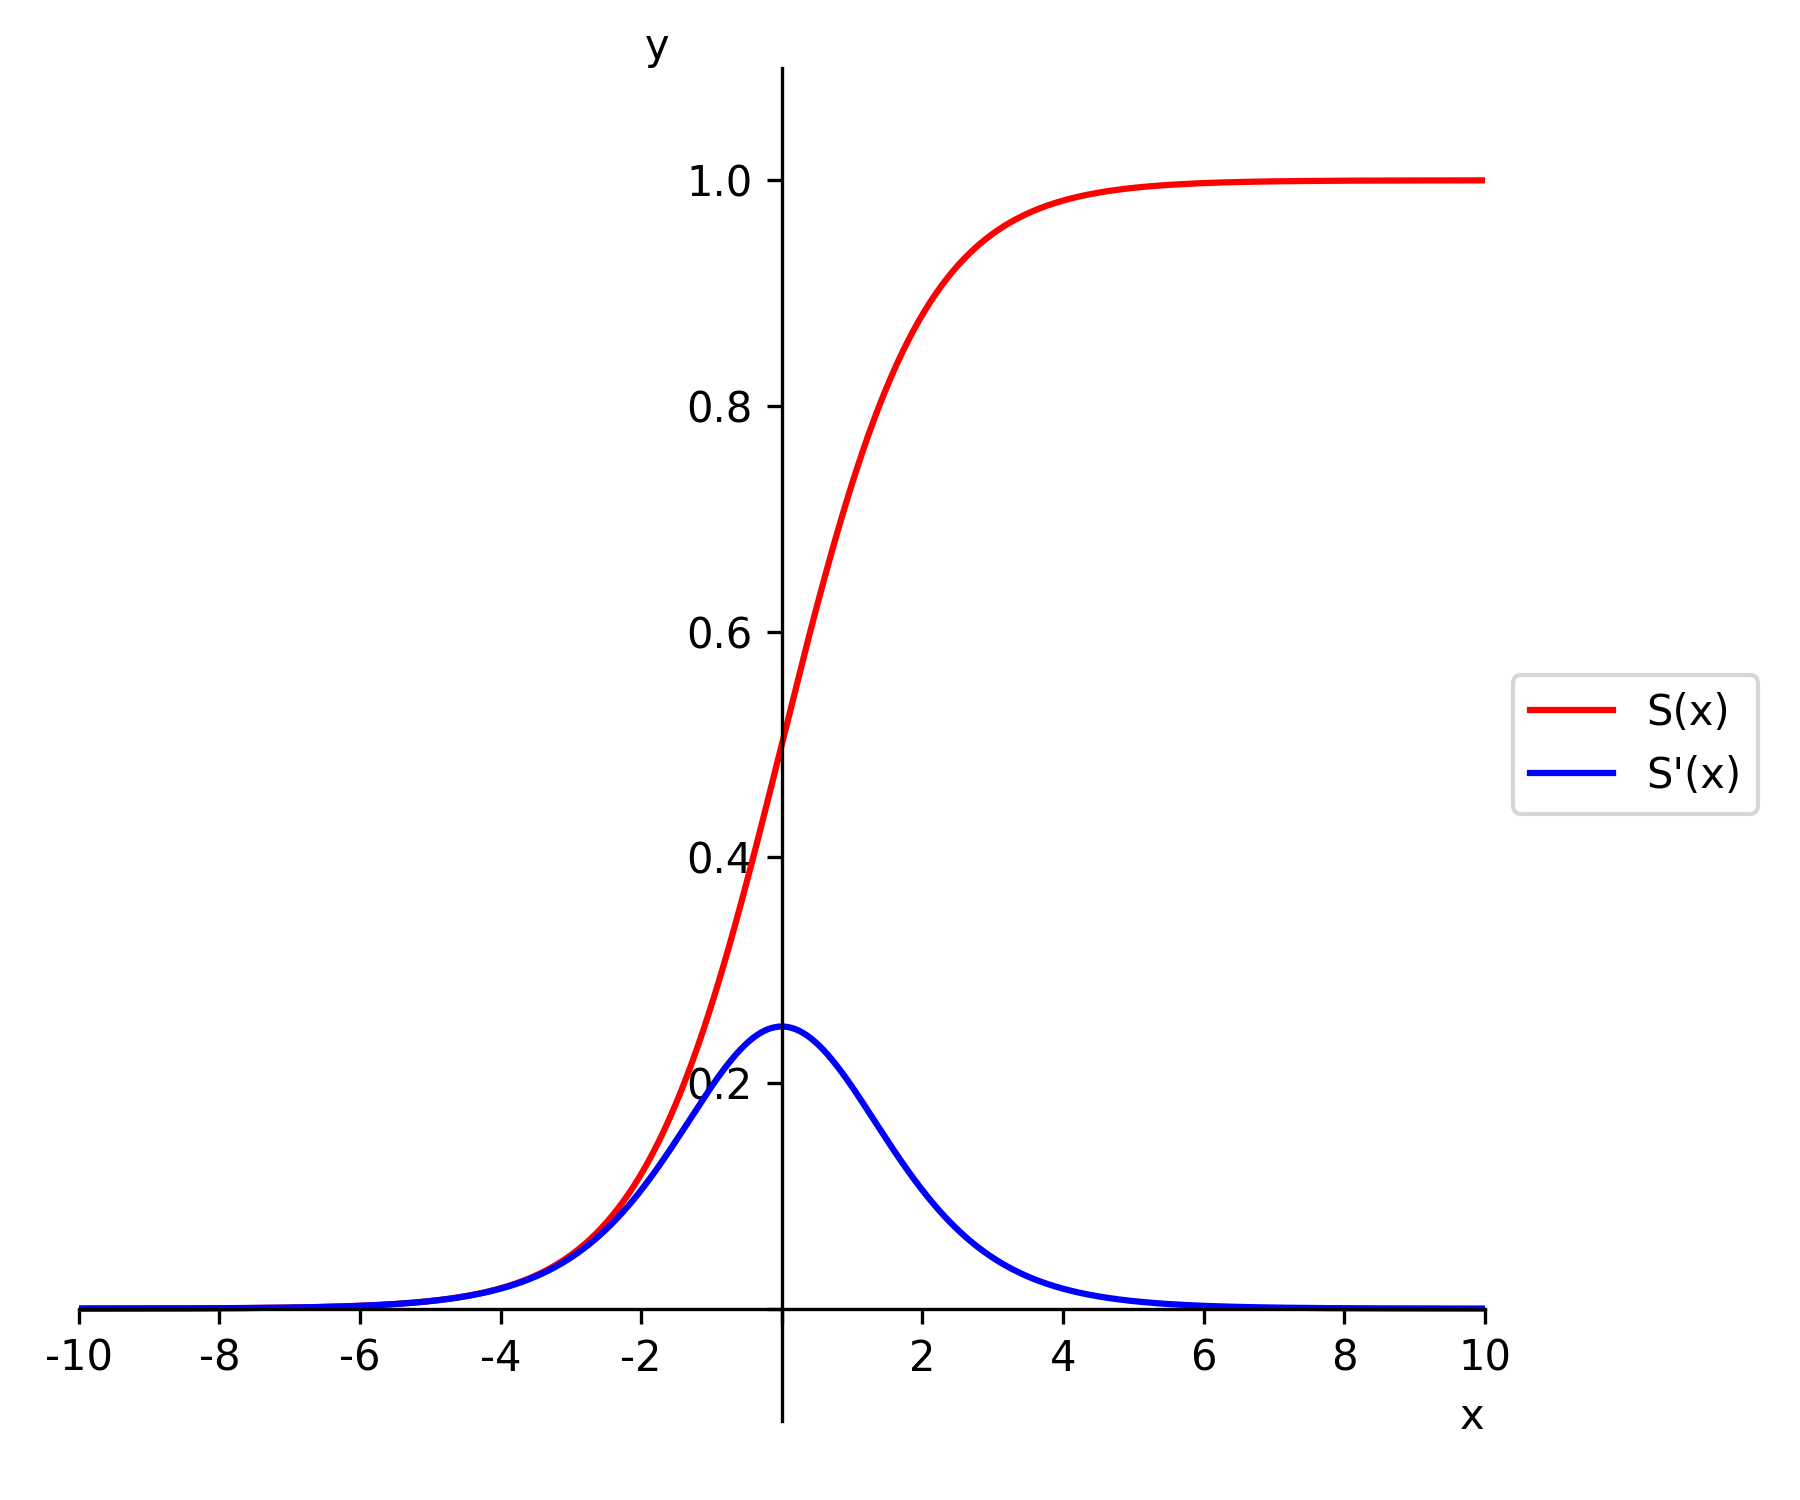
\includegraphics[width=1\linewidth]{Sigmoid_plus_derivative.png}
    \caption{Sigmoid function with derivative
    }
    \label{fig:Figure 4}
\end{figure}
%TC:endignore
As seen in Figure~\ref{fig:Figure 4}, a small derivative improves training stability. Every iteration of a sigmoid function results in small perturbations in network features. This increases the likelihood of convergence to loss minima without overshooting. This low rate of change, however, also increases the number of gradient descent steps needed to reach a minimum, increasing training time. 

Despite frequent use, sigmoid also possesses a vanishing gradient problem. Figure~\ref{fig:Figure 4} shows the derivative curve quickly becoming asymptotic towards zero. If neurons contain incredibly high or low feature values, their weights will not update significantly because of negligible derivatives. This results in improper model training, as certain weight dimensions remain unchanged and, therefore, unexplored during gradient descent.
%TC:ignore
\subsection{ReLU}
%TC:endignore
Contrasting the curve properties of sigmoid is ReLU, or Rectified Linear Unit, a piecewise function:
\begin{equation}
\label{relu}
R(x) = \begin{cases}
0,  x \leq 0 \\
x,  x > 0
\end{cases}
\end{equation}
%TC:ignore
\begin{figure}[H]
    \centering
    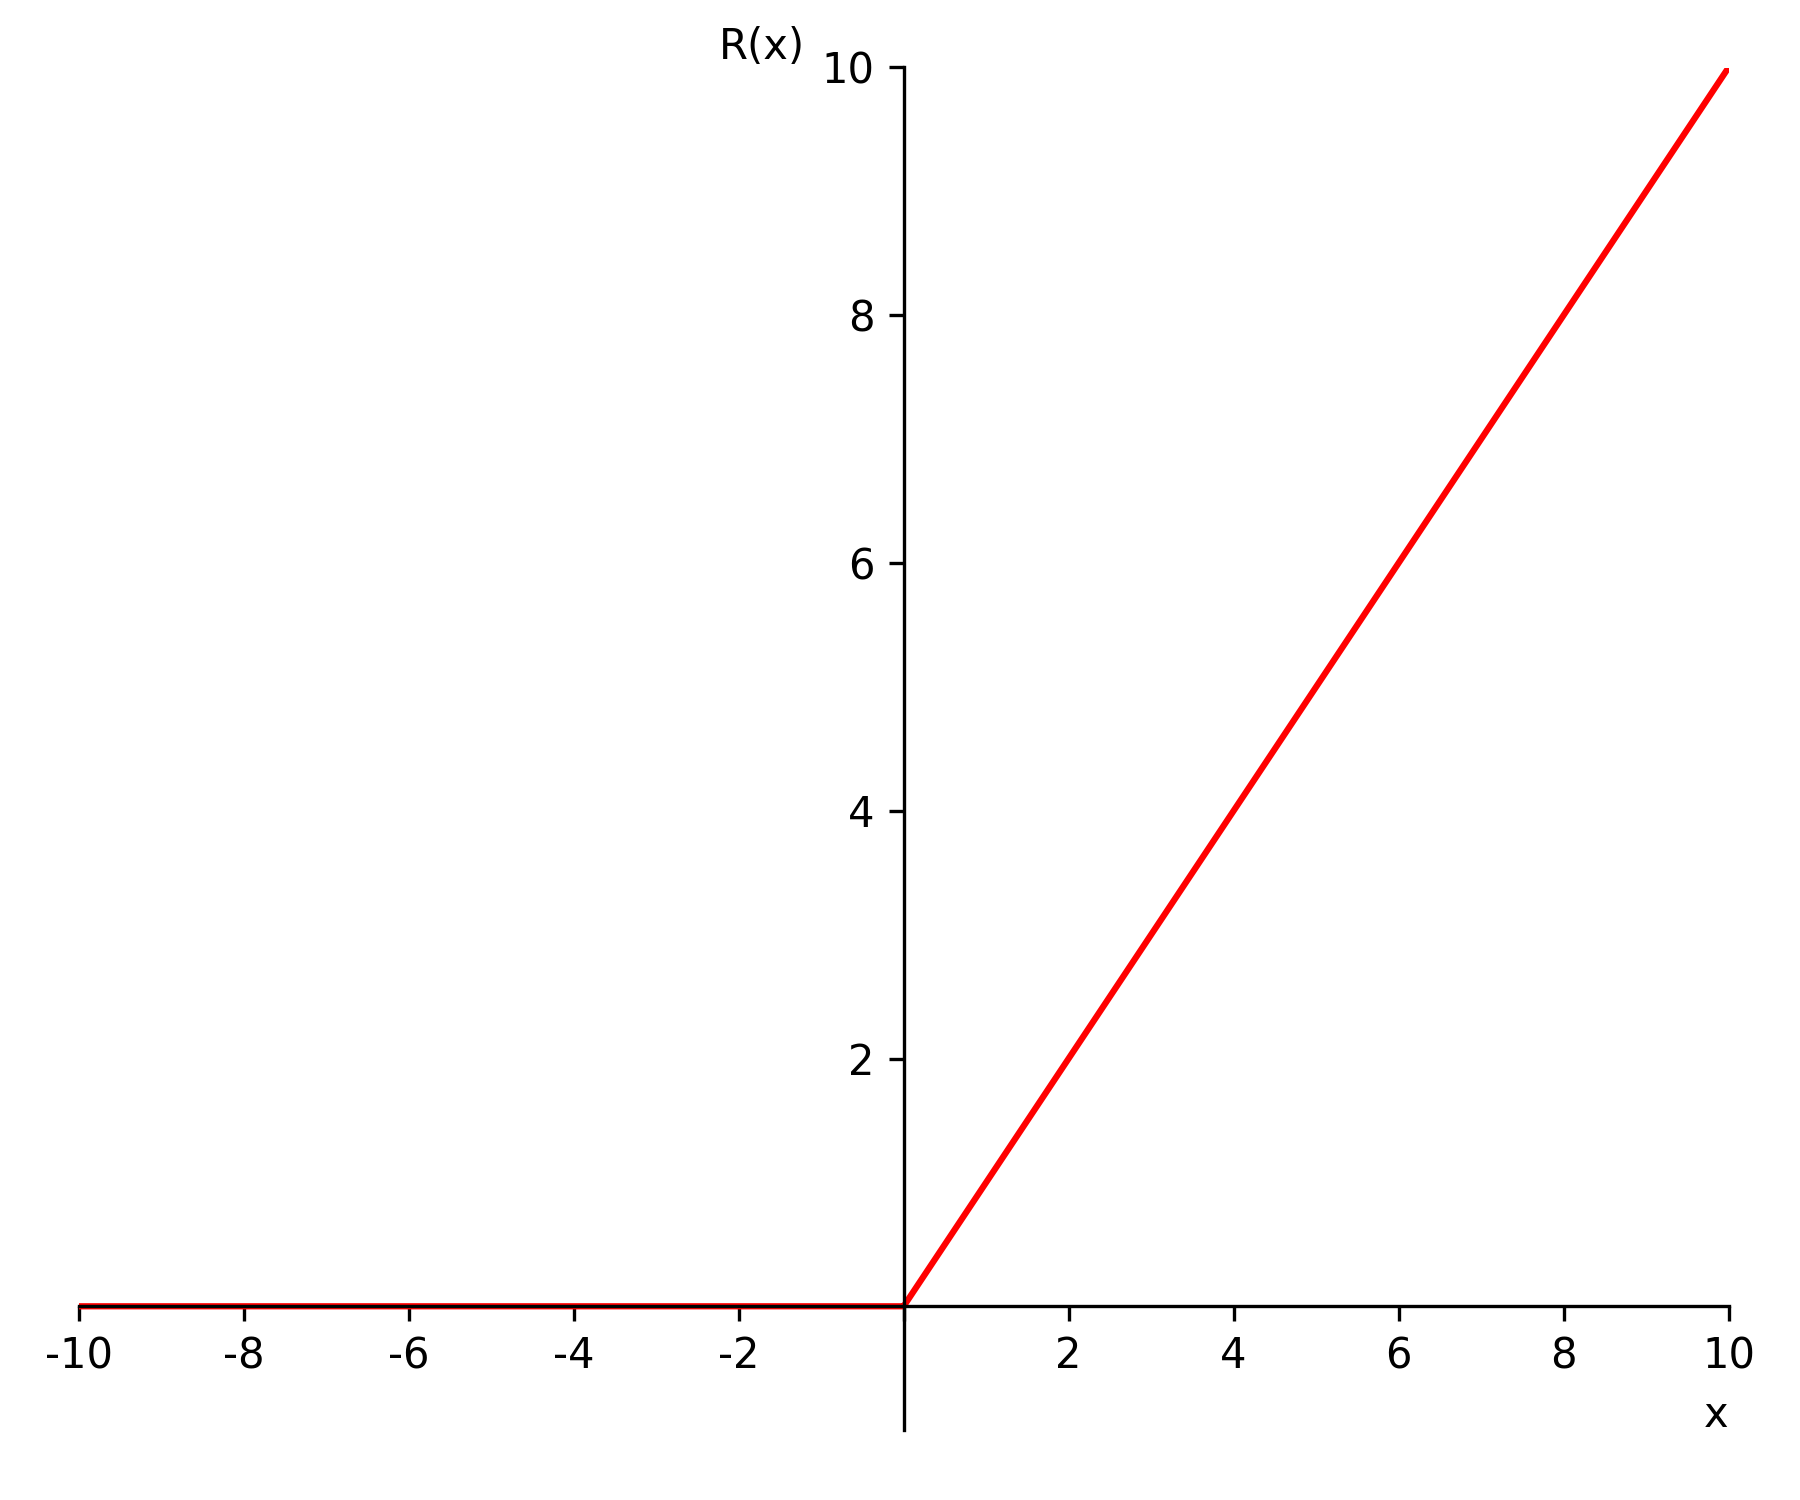
\includegraphics[width=1\linewidth]{ReLU.png}
    \caption{ReLU function}
    \label{fig:Figure 5}
\end{figure}
%TC:endignore
A simple linear function in the first quadrant, ReLU is a popular activation function because of its equal valuation of all feature types. No matter the magnitude of transformed data, a uniform derivative in Figure~\ref{fig:Figure 5} allows for explorations of all weight dimensions. Simultaneously, however, negation of the second quadrant in ReLU yields a dead neuron problem. While necessary for the function's non-linearity, treating all negative inputs as zero can reduce network robustness when features are negatively valued. Data normalization techniques avoids this issue, while most networks are applied in scenarios with positive-valued data. 
%TC:ignore
\section{Models for Analyzing Loss Landscapes}
\label{sec:loss_metrics}
\subsection{Hessian Matrix}
\label{sec:hessian}
%TC:endignore
In Section~\ref{sec:grad_desc}, the Jacobian matrix was key in analyzing loss gradients for descent to local minima. For a deeper analysis of function curvature which allows for this convergence, however, higher-order differential models are required. The Hessian matrix is used to compute second-order partial derivatives of the loss function with respect to all neural network weights.
\begin{definition}[Hessian Matrix]
\label{hessian}
    For a function $f : R^n \xrightarrow[]{} R$ where $x_i$ denotes the ith input, the Hessian matrix of $f$ is given by:
    \[
        H(f) =
        \begin{bmatrix}
        \frac{\partial^2 f}{\partial x_1^2} & \frac{\partial^2 f}{\partial x_1 \partial x_2} & \cdots & \frac{\partial^2 f}{\partial x_1 \partial x_n} \\
        \frac{\partial^2 f}{\partial x_2 \partial x_1} & \frac{\partial^2 f}{\partial x_2^2} & \cdots & \frac{\partial^2 f}{\partial x_2 \partial x_n} \\
        \vdots & \vdots & \ddots & \vdots \\
        \frac{\partial^2 f}{\partial x_n \partial x_1} & \frac{\partial^2 f}{\partial x_n \partial x_2} & \cdots & \frac{\partial^2 f}{\partial x_n^2}
        \end{bmatrix}
    \]
    When applied specifically to a neural network with loss function $C$ and weights $w_i$, we have:
    \[
        H(f) =
        \begin{bmatrix}
        \frac{\partial^2 C}{\partial w_1^2} & \frac{\partial^2 C}{\partial w_1 \partial w_2} & \cdots & \frac{\partial^2 C}{\partial w_1 \partial w_n} \\
        \frac{\partial^2 C}{\partial w_2 \partial w_1} & \frac{\partial^2 C}{\partial w_2^2} & \cdots & \frac{\partial^2 C}{\partial w_2 \partial w_n} \\
        \vdots & \vdots & \ddots & \vdots \\
        \frac{\partial^2 C}{\partial w_n \partial w_1} & \frac{\partial^2 C}{\partial w_n \partial w_2} & \cdots & \frac{\partial^2 C}{\partial w_n^2}
        \end{bmatrix}
    \]
\end{definition}
Though a superior measurement of function curvature, a Hessian model is implausible in real-life scenarios. For a neural network with $N$ weights, the Hessian matrix has dimensions of $N \times N$, holding $N^2$ variables. For networks with just thousands of parameters, microscopic by present standards, corresponding Hessian matrices have millions of values. For this reason, computing Hessians is space- and time-inefficient, forcing the matrix to act as just a theoretical indicator of loss curvature.

Instead, other techniques can approximate key features of the Hessian to reduce computational strain. One ubiquitous technique computes the eigenvalues of the matrix to understand the principal directions moved across a loss surface during gradient descent \cite{eigenintuition}. 
\begin{definition}[Eigenvalue]
\label{eigenvaluedefinition}
    Let $\Vec{x}$ denote an eigenvector. That is, a vector whose direction remains unchanged following a particular linear transformation $A$. An eigenvalue $\lambda$ represents a scale factor for $\Vec{x}$ after $A$ is applied. 
    Formally:
    \[
        A\Vec{x} = \lambda\Vec{x}
    \]
\end{definition}
The square nature of the Hessian allows for the existence of eigenvalues. Their relative sizes highlight the extent to which certain weight dimensions are stretched during gradient descent.
%TC:ignore
\subsection{Lipschitz Constant}
%TC:endignore
Another valuable loss approximation metric is a Lipschitz condition. Lipschitz functions have bounded distances between gradients which depend on distances between function outputs. This links to network stability by capturing exploding or diminishing gradients during training.
\begin{definition}[Lipschitz Condition]
    Assume a function $f : \mathbb{R}^2 \xrightarrow[]{} \mathbb{R}$ that is continuous and differentiable at every point. We have that:
    \begin{equation}
        \label{eq:lipcon}
        ||f(y) - f(x)||_2 \leq L ||y-x||_2
    \end{equation}
    Where $L$ represents a constant known as the Lipschitz constant and $||\alpha||_2$ represents the L2 norm operation. The L2 norm of a vector with $i$ elements is defined as:
    \[
        ||\alpha||_2 = \sqrt{{\alpha_1}^2 + {\alpha_2}^2 ... + {\alpha_i}^2}
    \]
\end{definition}
\begin{proof}
    Assume a function $f : \mathbb{R}^2 \xrightarrow[]{} \mathbb{R}$ that is continuous and differentiable on the interval $[a,b]$. By the Mean Value Theorem, we have:
    \[
        f'(c) = \frac{f(b)-f(a)}{b-a}
    \]
    Where $c$ is a point lying on the defined interval. Now assume a constant $L$ such that $L = max(f'(c))$. Substituting:
    \[
        \frac{f(b)-f(a)}{b-a} \leq L
    \]
    This theorem holds for scalar-valued functions. For extension to vectors, subtractions of vectors must be replaced with the L2 norm, which computes Euclidean distances (equivalent to subtractions) in vector spaces. This yields:
    \[
        \frac{||f(a)-f(b)||_2}{||b-a||_2} \leq L
    \]
    Rearranging:
    \[
        ||f(y) - f(x)||_2 \leq L ||y-x||_2 
    \]
    Matching the proposed definition in Equation~\ref{eq:lipcon}.
\end{proof}
Beyond just a bound, the Lipschitz constant relates to the Hessian matrix, as it is equal to the absolute value of the largest matrix eigenvalue.
\begin{proof}
    From Section~\ref{sec:hessian}, we know that the Hessian is a symmetric, real-valued matrix. Therefore, by the spectral theorem, the decomposition of a Hessian matrix $H$ is given by:
    \begin{equation}
        H = Q\Lambda Q^T
    \end{equation}
    Where $Q$ is an orthogonal matrix mapping standard bases to eigenvectors of $H$, and $\Lambda$ is a diagonal matrix containing eigenvalues of $H$ in descending order.
    Now, recall the Lipschitz condition, which states that:
    \[
        ||f(y) - f(x)||_2 \leq L ||y-x||_2 
    \]
    Suppose that $z = y-x$. Further assume function $f$ applies the Hessian matrix $H$ on a sample vector $z$. We have that:
    \[
        ||Hz||_2 \leq L ||z||_2 
    \]
    \[
        \frac{||Hz||_2}{||z||_2} \leq L
    \]
    Across all non-zero vectors $z$, the Lipschitz constant measures the maximum distance of outputs relative to inputs. Hence, it can be rewritten as:
    \[
        L = \sup_{z \, \neq \, 0} \frac{||Hz||_2}{||z||_2}
    \]
    Plugging in from our spectral decomposition:
    \[
        L = \sup_{z \, \neq \, 0} \frac{||Q \Lambda Q^T z||_2}{||z||_2}
    \]
    Matrix $Q$ and, by extension, $Q^T$ are orthogonal, preserving the length and therefore the L2 norm of vector $z$ post-transformation. Hence, they can be eliminated, yielding:
    \[
        L = \sup_{z \, \neq \, 0} \frac{||\Lambda z||_2}{||z||_2}
    \]
    Now recall that $\Lambda$ is a diagonal matrix of Hessian eigenvalues. Through matrix multiplication and application of the L2 norm, we have:
    \[
        L = \sup_{z \, \neq \, 0} \sqrt{\frac{\sum_{i=1}^n \lambda_i^2 z_i^2}{\sum_{i=1}^n z_i^2}}
    \]
    Squaring both sides for simplification:
    \[
        L^2 = \sup_{z \, \neq \, 0}\frac{\sum_{i=1}^n \lambda_i^2 z_i^2}{\sum_{i=1}^n z_i^2}
    \]
    Owing to its presence in both the numerator and denominator, the scaling of vector $z$ by any constant will cancel out. Hence, we assume vector $z$ to be a unit vector, yielding:
    \[
        L^2 = \sup\sum_{i=1}^n \lambda_i^2
    \]
    Finding the supremum in this case corresponds to the maximum squared eigenvalue of the matrix:
    \[
        L^2 = \max_i \lambda_i^2
    \]
    Finally:
    \[
        L = \max_i |\lambda_i|
    \]
    Therefore, spectral decomposition has unearthed a direct relation between the Lipschitz constant and the largest Hessian eigenvalue.
\end{proof}
%TC:ignore
\section{Methodology}
%TC:endignore
To experimentally address this essay's research question, a neural network has been developed and trained on real data. All experiments use the Python programming language (and auxiliary libraries) running in the Google Colab environment.
%TC:ignore
\subsection{Data Handling}
\label{sec:netdata}
%TC:endignore
To effectively analyze curvature metrics described in Section~\ref{sec:loss_metrics}, networks must be trained on a robust dataset. Here, an open-source wine quality dataset is used, which analyzes different chemical characteristics to rate wine on a scale of one to ten \cite{wine_quality_186}. This set contains numerous learnable parameters (such as wine pH, density, alcohol content, etc.) for a network to train on. Furthermore, it is suitable for binary classification (recall Definition~\ref{bclassdefinition}), as wines with ratings greater than six out of ten are considered high quality, while others are low quality.

% In order to prevent bias during network training, input features are subject to random shuffling. Each test case is also randomly assigned into training and validation groups, shown to the network at different stages of the training processes. Furthermore, with different data features having different magnitudes, normalization is required. Z-score scaling is used for all independent features, given by the formula:
% \begin{equation}
%     z = \frac{x - \mu}{\sigma}
% \end{equation}
% Where $x$ represents a specific feature value, and $\mu$ and $\sigma$ are the mean and standard deviation of the entire feature set respectively. Applying this technique gives each feature column a mean of zero and standard deviation of one, providing a uniform baseline from which independent features can be effectively compared (like wine pH versus density).

%TC:ignore
\subsection{Network Structure}
%TC:endignore
Post-normalization, training data is passed to a neural network created using the Pytorch library. A programmed training loop allows this network to repeatedly view all training examples, performing gradient descent with every pass-through.

In addition to activation functions, a neural network contains other tunable hyperparameters which must remain constant to avoid experimental interference. The hyperparameters corresponding to the highest network accuracy (see Section~\ref{sec:analytics}) are manually selected. A brief description of each one is given below:

\begin{table}[H]
    \centering
    \begin{tabularx}{\textwidth}{|X|X|X|}\hline
         Hyperparameter Name&  Role in Network& Name/Value\\\hline
         Hidden Layer Size&  Number of neurons in the intermediate layer between inputs and outputs& 32\\\hline
         Optimizer& Built-in algorithm that adaptively tunes gradient descent steps depending on weight values& Adaptive Moment Estimation\\\hline
         Learning Rate&  Scales size of gradient descent steps (see Equation~\ref{eq:gradient_descent}) & $5 \times 10^{-4}$\\\hline
         Number of Epochs & Number of times the entire dataset is shown to the network for training & 75 \\\hline
         Batch Size & Number of test cases shown to the network before a gradient descent step is taken & 64 \\\hline
    \end{tabularx}
    \caption{Description of Network Hyperparameters}
    \label{tab:Table 1}
\end{table}
\subsection{Analytics}
\label{sec:analytics}
After training, network performance is tested on a separate section of the dataset. Two metrics are used to evaluate model performance: raw loss and F1 scores. Raw loss represents the output of the network loss function detailed in Section~\ref{sec:lossfunc}. Improvements in training are seen with decreasing loss over epochs, highlighting network convergence onto a local minimum. Furthermore, to analyze effective classification (correct labeling of every wine as high or low quality), F1 scoring is implemented. This technique is superior to raw accuracy as it accounts for the imbalance of positive and negative classes in the dataset.

\begin{definition}[F1 Score]
    An F1 score harmonically evaluates a model's precision and recall, given by the formula:
    \[
        F_1 = \frac{TP}{TP + \frac{1}{2} (FP + FN)}
    \]
    Where $TP$ represents true positives, $FP$ false positives, and $FN$ false negatives.
\end{definition}

For computation of the maximum Hessian eigenvalue, the power iteration technique is used. This algorithm randomly samples directions within the Hessian, tracking eigenvalues until likely that a maximum has been found.

\begin{definition}[Power Iteration]
    Assume a Hessian matrix $H \in \mathbb{R}^{m \times m}$, and a random vector $v^0 \in \mathbb{R}^m$. Any vector in this space can be decomposed into a linear combination of Hessian eigenvectors, yielding:
    \[
        v^0 = c_1e_1 + c_2e_2 ... + c_ne_n
    \]
    Where $c_i$ is a scalar and $e_i$ is a linearly independent eigenvector. Now, assume the Hessian matrix $H$ multiplies this random vector $v^0$:
    \[
        Hv^0 = c_1He_1 + c_2He_2 ... + c_nHe_n
    \]
    Substituting, using the definition of an eigenvalue (see Section~\ref{eigenvaluedefinition}):
    \[
        Hv^0 = c_1\lambda_1e_1 + c_2\lambda_2e_2 ... + c_n\lambda_ne_n
    \]
    Where $\lambda_1 > \lambda_2$ and so on. Let us again multiply this equation by the Hessian:
    \[
        H^2v^0 = c_1H\lambda_1e_1 + c_2H\lambda_2e_2 ... + c_nH\lambda_ne_n
    \]
    Again, by substitution, we have:
    \[
        H^2v^0 = c_1\lambda_1^2e_1 + c_2\lambda_2^2e_2 ... + c_n\lambda_n^2e_n
    \]
    After multiplying this expression by the Hessian $k$ times, we have:
    \[
        H^kv^0 = c_1\lambda_1^ke_1 + c_2\lambda_2^ke_2 ... + c_n\lambda_n^ke_n
    \]
    Rearranging:
    \[
        H^kv^0 = \lambda_1^k (c_1e_1 + c_2{\left(\frac{\lambda_2}{\lambda_1}\right)}^ke_2 ... + c_n{\left(\frac{\lambda_n}{\lambda_1}\right)}^ke_n)
    \]
    With $\lambda_1$ representing the maximum eigenvalue, other eigenvalues will become negligible for a significantly large $k$. This allows us to make the approximation:
    \[
        H^kv^0 \approx \lambda_1^k (c_1e_1)
    \]
    Therefore isolating the largest matrix eigenvalue.

    Additionally, interference is tracked by measuring the Lipschitz constant of neural network outputs with respect to its inputs. This helps identify the extent to which model inputs influence gradients independent of weight settings. A theoretical upper bound is calculated using the singular values of the weight matrix. A first-order Lipschitz relationship is also calculated by sampling the Jacobian matrix to analyze variance in network gradients with training.
\end{definition}
%TC:ignore
\section{Results}
%TC:endignore
Instantiation of two distinct neural networks, running the sigmoid and ReLU activation functions on the same dataset, has yielded the below results.
\subsection{Conclusions}
\label{sec:conclusion}
Experiments resulted in both sigmoid and ReLU networks minimizing loss. The figures below highlight how ReLU significantly outperformed sigmoid on both the training and validation datasets. In addition to lowered loss, the network using ReLU reached its minimum quicker than sigmoid (most notably in Figure~\ref{fig:Figure 7}), suggesting that larger activation gradients motivate time-efficient training.
%TC:ignore
\begin{figure}[H]
    \centering
    \begin{minipage}{0.5\textwidth}
        \centering
        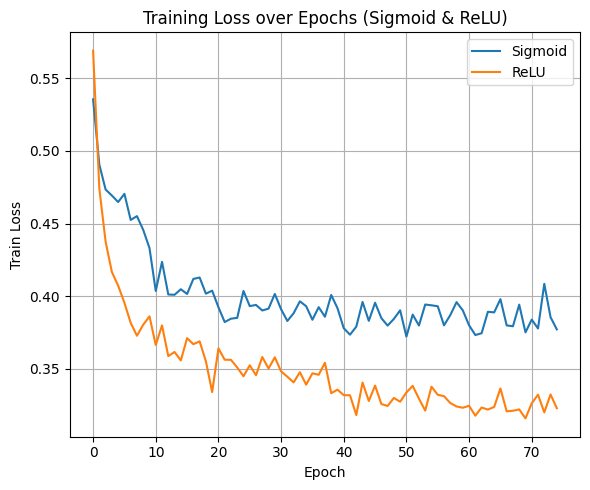
\includegraphics[width=1\textwidth]{Sigmoid & ReLU Smoothed Training Loss.png} % first figure itself
        \caption{Training Loss Curves}
        \label{fig:Figure 6}
    \end{minipage}\hfill
    \begin{minipage}{0.5\textwidth}
        \centering
        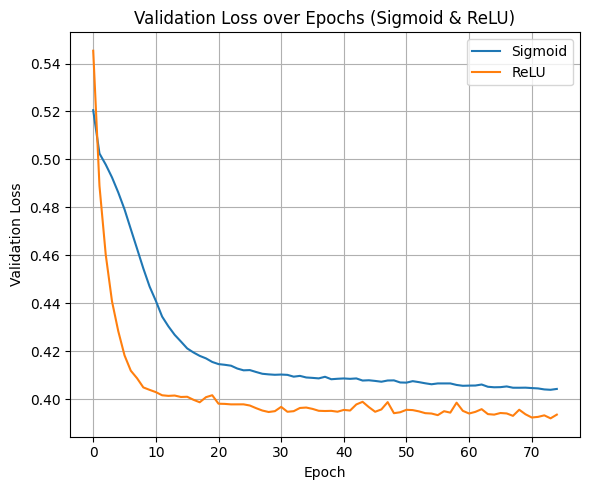
\includegraphics[width=1\textwidth]{Sigmoid & ReLU Validation Loss.png} % second figure itself
        \caption{Validation Loss Curves}
        \label{fig:Figure 7}
    \end{minipage}
\end{figure}
%TC:endignore
Despite varying loss curves, both activation functions have similar F1 scores. Although ReLU predicts classification probabilities more confidently, both sigmoid and ReLU predict with similar precision and recall accuracies. ReLU's efficiency trend is further observed, as it reaches its F1 optimum far earlier than sigmoid.
%TC:ignore
\begin{figure}[H]
    \centering
    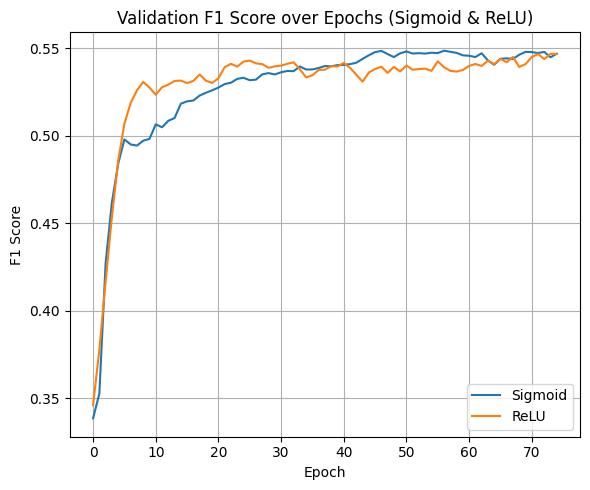
\includegraphics[width=0.6\textwidth]{Sigmoid & ReLU F1 Score.png} % first figure itself
    \caption{Validation F1 Score Curves}
    \label{fig:Figure 8}
\end{figure}
%TC:endignore
Interestingly, the second-order trends for both activation functions largely varied, as seen in Figure~\ref{fig:Figure 9}:
%TC:ignore
\begin{figure}[H]
    \centering
    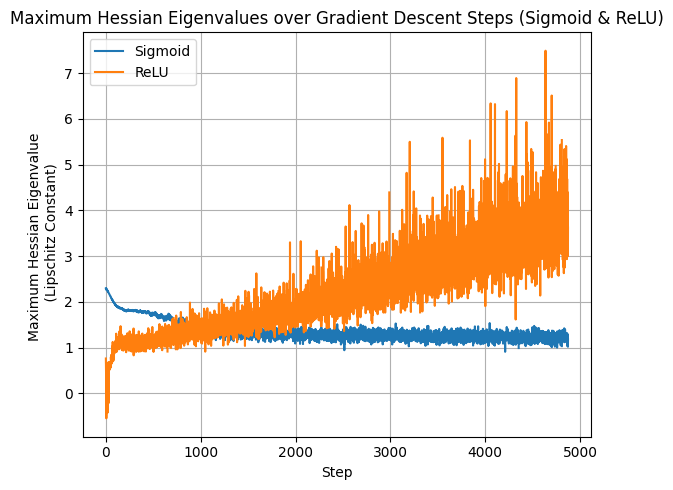
\includegraphics[width=0.8\textwidth]{Sigmoid & ReLU Max Hessian Eigenvalue.png} % first figure itself
    \caption{Maximum Hessian Eigenvalue Curves}
    \label{fig:Figure 9}
\end{figure}
%TC:endignore
For sigmoid, Figure~\ref{fig:Figure 9} shows initially steep eigenvalue changes. This highlights more movement across the loss surface for optimization. Decreases in the maximum eigenvalue suggest that the loss surface becomes less curved as training progresses. Furthermore, convergence of the maximum eigenvalue to the value of one strongly suggests that the sigmoidal network has found a minimum with negligible local curvature. Small fluctuations emphasize training stability during gradient descent, with the network making fewer abrupt directional changes across the loss surface to find its minimum.

Figure~\ref{fig:Figure 9} illustrates an opposite trend for ReLU. The maximum eigenvalue being negative at the start of training shows an incredibly peculiar loss surface, with the network initially attempting to move away from local minima to optimize. This suggests an unstable training environment, likely due to large gradients in an unbounded activation function. Instability is further observed with large eigenvalue fluctuations throughout training. As training stabilizes, an increasing trend shows an increase in curvature, making the loss surface steeper. Rather than quickly settling on a local minimum, this highlights how the ReLU network aggressively explores the loss surface to optimize. 

These conclusions are further confirmed by the first-order trends observed in Figure~\ref{fig:Figure 10}:
%TC:ignore
\begin{figure}[H]
    \centering
    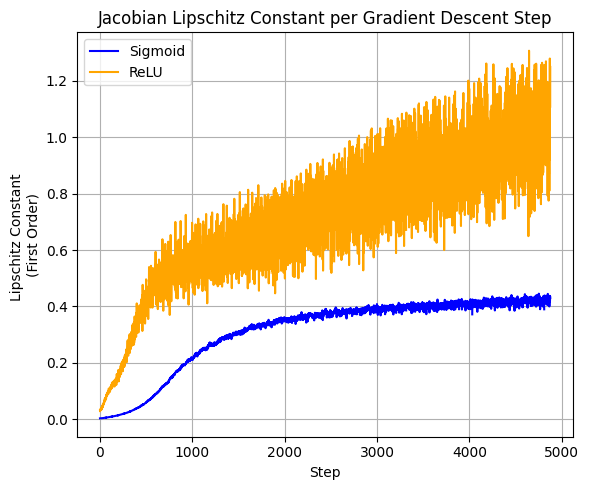
\includegraphics[width=0.8\textwidth]{Sigmoid and ReLU Jacobian Lipschitz.png} % first figure itself
    \caption{Lipschitz Constant of Gradient Curves}
    \label{fig:Figure 10}
\end{figure}
%TC:endignore
This graph encapsulates ReLU's increasing gradients, as the gradient Lipschitz constant continues to increase with training. Conversely, the leveling of sigmoid's Lipschitz constant highlights how vanishing gradients prevent significant model updates towards the end of training. 

Overall, sigmoidal networks sacrifice speed for training stability, allowing for slow convergence to a local minimum. Conversely, the ReLU network aggressively explored the loss surface in an efficient yet increasingly unstable manner. Though both activation functions affected loss surface curvature differently, their loss minimization and similar F1 scores highlight how varying neural network architectures can be suitable for solving similar problems.
%TC:ignore
\subsection{Model Errors}
%TC:endignore
The sigmoid and ReLU networks both demonstrated classification accuracies of roughly 80\% on validation data, leaving notable room for improvement. Numerous false positives were predicted, with the contingency matrix below showing the false positive mispredictions of both models relative to one another.

% This is understandable, given that the models had simplistic architectures and were trained on a relatively small data set.

% Both models sacrificed precision for recall, ensuring that a larger proportion of positive predictions were made. This is exemplified by their optimal F1 scoring threshold of 0.2. The threshold being significantly less than the median of probabilities (0.5) highlights the models' tendencies to predict positively. Though this leads to more true positive predictions, a low threshold also forces a correspondingly high number of false positives.

\begin{table}[H]
    \centering
    \begin{tabular}{|c|c|c|}
        \hline
        \multicolumn{3}{|c|}{False Positive Network Predictions} \\
        \hline
         & ReLU & $\neg$ReLU \\
        \hline
        Sigmoid & 157 & 32 \\
        \hline
        $\neg$Sigmoid & 61 & 790 \\
        \hline
    \end{tabular}
    \caption{False Positives Contingency Matrix}
    \label{tab:fp_matrix}
\end{table}

As seen in Table~\ref{tab:fp_matrix}, many of the same test cases were misclassified by both networks, suggesting that the training data contained difficult learnable examples. Being more robust, ReLU had a stronger recall than sigmoid, thereby classifying more false positives.

In comparison, both networks rarely predicted false negatives, as seen in Table~\ref{tab:fn_matrix}: 
\begin{table}[H]
    \centering
    \begin{tabular}{|c|c|c|}
        \hline
        \multicolumn{3}{|c|}{False Negative Network Predictions} \\
        \hline
         & ReLU & $\neg$ReLU \\
        \hline
        Sigmoid & 30 & 30 \\
        \hline
        $\neg$Sigmoid & 14 & 966 \\
        \hline
    \end{tabular}
    \caption{False Negatives Contingency Matrix}
    \label{tab:fn_matrix}
\end{table}
Overlapping mislabelings again suggest the presence of intrinsically difficult classification examples within the dataset. Furthermore, ReLU's aggressive positive prediction tendency ensures fewer false negatives than sigmoid.

% Overall, further development and fine-tuning are required to improve model performance regardless of the activation function. Gradient descent techniques like Momentum and Dropout can improve both models' robustness, leading to better classification of difficult test cases. Furthermore, a deeper search for an optimal threshold can better balance model precision and recall, improving both F1 scores and raw accuracy. 

%TC:ignore
\subsection{Experimental Improvements}
%TC:endignore

Despite a controlled training environment, improvements in experimental setup can yield more objective results. This essay's experiments contain sample bias, as only one network instance was trained for both sigmoid and ReLU. An average of multiple experimental trials would solidify results, even at the expense of storage space and compute time. 

Training on a larger number of varied datasets would improve the binary classification potential of each activation function. Furthermore, certain activation functions may intrinsically improve the fit on certain datasets. Even input features can impact model performance, as seen below:

%TC:ignore
\begin{figure}[H]
    \centering
    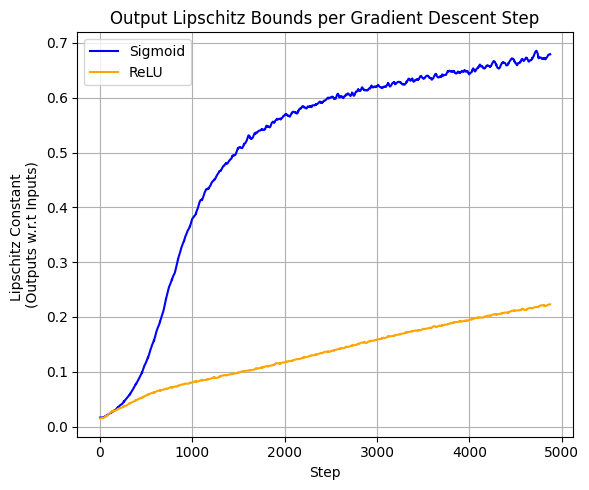
\includegraphics[width=0.7\textwidth]{Sigmoid & ReLU Output Lipschitz.png} % first figure itself
    \caption{Lipschitz Constant of Model Outputs}
    \label{fig:Figure 11}
\end{figure}
%TC:endignore

Figure~\ref{fig:Figure 11} illustrates how the Lipschitz constant of model outputs with respect to inputs grows differently in sigmoid and ReLU during training. Testing on other datasets can help negate this feature-specific interference, ensuring that only model parameters contribute to the differences observed in both activation functions. 

% Random data shuffling during training prevented model memorization of non-generalizable patterns. Different random seeds for each activation function's network, however, initialized weights and biases at different locations on the loss surface. This initially random yet varied placement may already have optimized one network's parameters relative to the other, rendering it easier to find a local minimum. 

% Finally, hyperparameter tuning was only performed using sigmoid as the activation function. Model performance is therefore slightly disadvantaged when using ReLU, as the function interacts with hyperparameters differently. Surprisingly, ReLU still outperformed sigmoid in loss minimization (see Section~\ref{sec:conclusion}), justifying its ubiquity in present-day neural networks.
%TC:ignore
\section{Extension}
%TC:endignore
Binary classifiers are generations behind in performance and architecture compared to modern-day neural networks. For example, Natural Language Processing (NLP) and image generation models like ChatGPT and Midjourney utilize more complex and deep structures. Still, this essay's research question remains valid as every neural network, regardless of size and complexity, requires an activation function. Methods used in this work provide key insights into any network's performance, yet their practicality diminishes with network size. For advanced modern networks, tracking second-order relationships (like Hessian eigenvalues) is computationally inefficient, even by use of approximation techniques. First-order metrics, however, like Lipschitz constants of outputs and Jacobians, continue to provide valuable analytics.

The techniques applied in this essay can be extended to analyze activation functions during multi-class classification. Additionally, these same techniques can be applied to other network architectures, like transformers and attention modules used in Large Language Models (LLMs). Within these architectures, the impacts of other hyperparameters on loss surfaces can also be analyzed, preventing the manual and arbitrary fine-tuning done by most AI developers. Overall, future exploration of techniques in this essay can help optimize a technology that has already pushed our limits of data-driven automation and our understanding of machine intelligence.
%TC:ignore
\textcolor{white}{QED.}
%TC:endignore
\printbibliography
\end{document}
